\section{Apache Spark} \label{spark}
Apache Spark\footnote{Apache Spark:  \href{https://spark.apache.org}{https://spark.apache.org}} nasce come un progetto di ricerca al \href{https://amplab.cs.berkeley.edu/}{UC Berkeley AMPLab} nel 2009 per poi essere reso pubblico sotto forma di progetto open source nel 2010. Acquistato dall'Apache Software Foundation nel 2013, ad oggi è uno dei framework più utilizzati nel campo delle elaborazioni distribuite di grandi quantità di dati, con alle spalle una comunità di centinaia di sviluppatori e centinaia di organizzazioni.
\subsection{Cosa è Spark}
Apache Spark è un motore multilingue per la automazione di ingegneria dei dati, scienza dei dati e apprendimento automatico su macchine a nodo singolo o cluster. La peculiarità di Apache Spark è la sua capacità di elaborare set di dati di grandi dimensioni in maniera efficiente, distribuendo attività di elaborazione dati su più computer, anche integrando Hadoop YARN e HDFS. Questi attributi sono fondamentali per il mondo dei big data e del machine learning.

All'epoca della nascita di questo progetto, Hadoop MapReduce era il motore di programmazione parallela predominante per i cluster, essendo il primo sistema open source ad affrontare l'elaborazione dei dati su migliaia di nodi. L'AMPlab aveva lavorato con molti dei primi utenti di MapReduce per capire i benefici e gli svantaggi di questo nuovo modello di programmazione ed era quindi in grado di sintetizzare una lista di problemi attraverso diversi casi d'uso e iniziare a progettare piattaforme di calcolo più generali. Spark pertanto nasce prendendo i pregi di MapReduce ed introducendo nuove funzionalità che, ad oggi, lo hanno reso uno dei framework più solidi nell'ambito dei big data:
\begin{itemize}
    \item Spark supporta l’elaborazione in memoria centrale per migliorare le prestazioni delle applicazioni, a differenza di MapReduce che deve riportare i dati sul disco dopo ogni azione Map o Reduce.
    \item Il suo predecessore poteva essere implementato soltanto utilizzando il linguaggio Java. Spark, invece, fornisce connessioni native per i linguaggi di programmazione Java, Scala, Python e R e supporta operazioni SQL. 
    \item Può elaborare grafi ed è anche dotato di una propria libreria di machine learning. Grazie alle sue alte prestazioni, è possibile utilizzarlo sia per l'elaborazione in batch sia per l'elaborazione simil real-time. 
    \item Sfrutta il paradigma del Transfer Learning (il riutilizzo di un modello pre-addestrato su un nuovo problema). 
    \item Permette di elaborare dei dati da vari repository come Hadoop Distributed File System (HDFS), database NoSQL e Apache Hive utilizzando le API di storage di dell'ecosistema Hadoop.
    \item In MapReduce, ogni operazione è indipendente dall'altra e Hadoop non ha idea di quale verrà dopo. Spark, invece, utilizza un modello di programmazione completamente innovativo basato su grafi diretti aciclici (DAGs).
\end{itemize}

\subsection{Architettura}
L'architettura di Apache Spark si ispira fortemente a quella di Hadoop. Difatti, presenta una struttura gerarchica \textbf{Master-Slaves} dove il nodo master che gestisce i nodi in esecuzione e controlla l’amministratore del cluster. 

All'interno del nodo master viene istanziato un \textit{driver}, processo che si occupa di distribuire il codice dell’utente tra i nodi e convertirlo in più attività (\textit{jobs}). Il driver distribuisce questi compiti sui nodi slave (worker) e organizza la loro esecuzione.  Le applicazioni Spark vengono eseguite come serie indipendenti di processi in ambiente distribuito, coordinate dallo \textbf{SparkContext}, un processo che funziona come una porta d'accesso a tutte le funzionalità di Spark.

I \textbf{nodi worker} eseguono le attività assegnate dal driver su questi nodi. Eseguti i jobs assegnati, restituiscono il risultato allo SparkContext. 
È però necessario implementare un gestore del cluster o \textbf{cluster manager} (Spark Standalone Cluster Manager, Hadoop Yarn, Apache Mesos, Kubernetes) per mediare tra i workers e driver. 
\begin{figure}[hbt!]
    \centering
    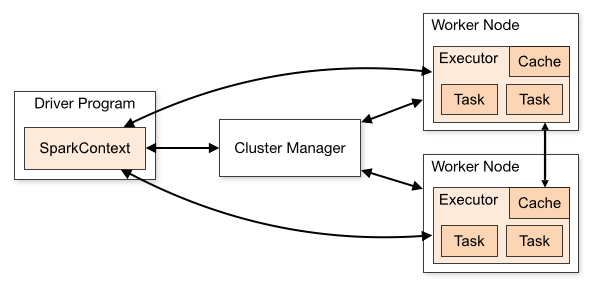
\includegraphics[width=1\textwidth]{img/sparkarchitecture.png}
    \caption{Architettura Spark}
    \label{fig:spark_architettura}
\end{figure}\\

% Spark può essere eseguito in due modalità:
% \begin{itemize}
%     \item \textbf{Cluster Mode}: il cliente che presenta l'applicazione Spark avvierà il driver e manterrà lo SparkContext. Quindi, fino a quando l'esecuzione del lavoro non sarà finita, la gestione dei jobs sarà svolta dal driver. Inoltre, il client deve rimanere sempre in contatto con il cluster: il client dovrà essere online fino a quando quel particolare processo non sarà completato.
%     \item \textbf{Client Mode}: il driver Spark o il master dell'applicazione Spark verrà avviato in una qualsiasi delle macchine worker. Quindi, il client che sta presentando l'applicazione può presentare l'applicazione e può o andare via dopo aver avviato l'applicazione o continuare con qualche altro lavoro. Questo meccanisco è anche chiamato \textit{Fire and Forget}.
% \end{itemize}
\subsection{Spark RDD e DataFrame} \label{rdd_df}
Il motore Spark usa principalmente set di \textit{Resilient Distributed Dataset (RDD)} come tipo di dati sottostante. Gli RDD sono raccolte di elementi a tolleranza di errore che possono essere distribuiti tra più nodi in cluster e lavorati in parallelo. Hanno una struttura progettata per nascondere la complessità computazionale agli utenti: non hanno bisogno di definire dove vengono inviati file specifici, quali risorse di calcolo verranno utilizzate per archiviare o recuperare i file. Sono altamente resilienti, cioè sono in grado di superare rapidamente qualsiasi problema poiché gli stessi pezzi di dati sono replicati su più nodi esecutori, così, anche se un nodo fallisce, un altro elaborerà comunque i dati.

Ci sono due modi per creare RDD - parallelizzando una collezione esistente nel programma driver, o facendo riferimento a un set di dati in un sistema di storage esterno, come un file system condiviso, HDFS, HBase, ecc. Con gli RDD, si possono eseguire due tipi di operazioni:
\begin{itemize}
    \item \textbf{Transformations}: prendono RDD come input e producono uno o più RDD come output. Ogni volta creano un nuovo RDD poiché essi sono immutabili. 
    \item \textbf{Actions}: operazioni Spark RDD che danno valori non RDD. I valori dell'azione sono memorizzati nel driver o nel sistema di archiviazione esterno. Un'azione è uno dei modi per inviare dati da Executer al driver.
\end{itemize}
\begin{figure}[hbt!]
    \centering
    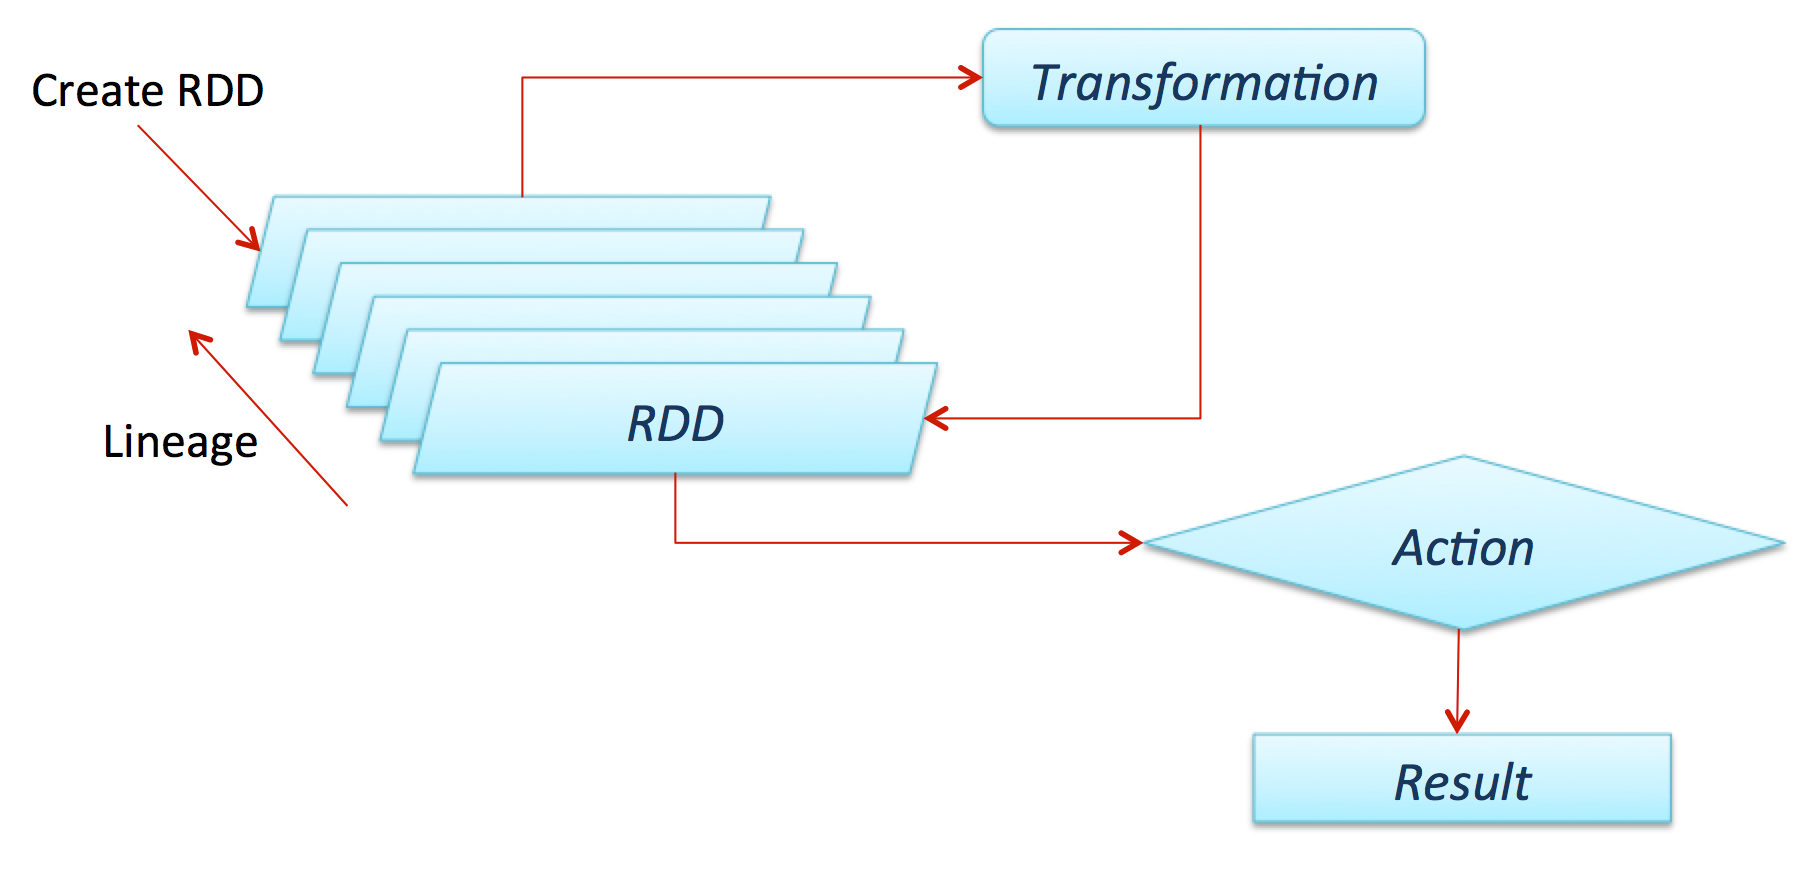
\includegraphics[width=1\textwidth]{img/spark_rdd.png}
    \caption{Operazioni su RDD}
    \label{fig:spark_rdd}
\end{figure}

Nel progetto di Tesi è stato però utilizzato un altro tipo astrazione presente in Spark per memorizzare dati, i \textit{DataFrame}. Sono implementati come degli RDD, pertanto sono anch'essi una collezione di dati distribuiti. La differenza sta nel fatto che sono organizzati in colonne nominate, come avviene nelle tabelle dei database relazionali. Un'altra caratteristica di DataFrame è che le operazioni sono ottimizzabili da Spark mentre le operazioni su RDD sono imperative e passano attraverso le trasformazioni e le azioni in ordine. Questo perfezionamento viene eseguito da un ottimizzatore di query, \textit{Catalyst Optimizer}, che supporta sia l'ottimizzazione basata sulle regole che quella basata sui costi. Nell'ottimizzazione basata su regole, usa un insieme di regole per determinare come eseguire la query. L'ottimizzazione basata sul costo trova il modo più adatto per eseguire l'istruzione. Nell'ottimizzazione basata sui costi, vengono generati più piani utilizzando le regole e poi viene calcolato il loro costo.
\begin{figure}[hbt!]
    \centering
    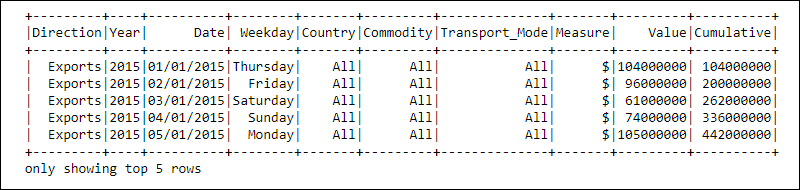
\includegraphics[width=1\textwidth]{img/dataframe_example.png}
    \caption{Esempio di struttura di un DataFrame}
    \label{fig:dataframe_example}
\end{figure}

Durante la fare di sperimentazione, sono stati utilizzati DataFrame per memorizzare i record presenti nei dataset ed effetturare operazioni su di essi. I DataFrame sono stati popolati utilizzando metodi implementati all'interno della struttura dati che permettono di estrarre informazioni da file di diversi formati. Nello specifico sono stati utilizzati per leggere dati da file in formato CSV e CoNLL '03.
\subsection{Directed Acyclic Graphs in Spark}
Con tutti i vari job, Spark crea un flusso logico di operazioni, che è noto come \textbf{Directed Acyclic Graph (DAG)}. In Spark, un DAG è un grafo diretto aciclico dove i \textit{vertici} rappresentano le strutture dati (RDD o DataFrame) e gli \textit{archi} rappresentano l'operazione da applicare su di esse. Alla chiamata di un'azione, il DAG creato viene sottoposto al \textit{DAGScheduler} che divide ulteriormente il grafo nelle fasi da svolgere per portare a termine il compito. Questo aiuta a: ridurre al minimo il rimescolamento dei dati, ridurre la durata dei calcoli, migliorare l'efficienza del processo nel tempo.

Inoltre, Spark sfrutta la strategia denominata \textbf{lazy evaluation}, ovvero posticipa la valutazione di un'espressione finché non è necessaria. Per le trasformazioni, Spark le aggiunge a un DAG e solo quando il driver richiede alcuni dati, questo DAG viene effettivamente eseguito. Ciò significa che, memorizzando ogni dettaglio delle operazioni eseguite su diverse partizioni di RDD, è possibile recuperare facilmente dati persi in caso di fallimento o di perdita di qualsiasi RDD.
\begin{figure}[hbt!]
    \centering
    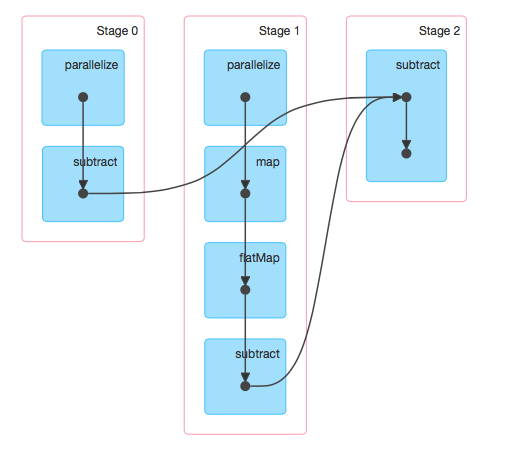
\includegraphics[width=0.8\textwidth]{img/sparkdag.png}
    \caption{Esempio di Spark DAG}
    \label{fig:spark_dag}
\end{figure}


\subsection{Spark Core}
Spark Core è la base dell'intero progetto: fornisce il dispacciamento distribuito dei compiti, lo scheduling e le funzionalità I/O di base. Spark Core funziona in parte come un livello API. Oltre al motore Spark Core, l’ambiente API Apache Spark viene fornito insieme ad alcune librerie da utilizzare nelle applicazioni di analisi dei dati.
\begin{itemize}
    \item \textbf{Spark SQL}: è un modulo Spark per l'elaborazione di dati strutturati. A differenza delle API di base di Spark RDD, le interfacce fornite da Spark SQL forniscono a Spark più informazioni sulla struttura dei dati e sul calcolo che viene eseguito. Internamente, Spark SQL utilizza queste informazioni extra per eseguire ottimizzazioni. Dato che quando si calcola un risultato, viene utilizzato lo stesso motore di esecuzione, indipendentemente da quale API/linguaggio si sta utilizzando, gli sviluppatori possono facilmente fare avanti e indietro tra diverse API a loro piacimento. DataFrame fa parte di questa libreria.
    \item \textbf{Spark Streaming}: una libreria per l'elaborazione scalabile, ad alta velocità e fault-tolerant di flussi di dati in tempo reale.  I dati possono essere ottenuti da molte fonti come Kafka, Kinesis, o socket TCP, possono essere elaborati tramite algoritmi di Machine Learning ed elaborazione grafica ed infine possono essere inviati a file system, database e dashboard live.
    \item \textbf{MLlib}: una libreria di Machine Learning (ML) il cui scopo è di rendere l'apprendimento automatico facile e scalabile. Essa mette a disposizione algoritmi di Machine Learning, Pipelines e diversi altri strumenti per lo svolgimento di operazioni statistiche avanzate sui dati e per creare applicazioni attorno a queste analisi.
    \item \textbf{GraphX}: è un nuovo componente di Spark per i grafi e il calcolo parallelo su di essi. Per supportare il calcolo dei grafi, GraphX mette a disposizione un insieme di operazioni fondamentali (ad esempio, \textit{subgraph}, \textit{joinVertices}, e \textit{aggregateMessages}). Inoltre, include una crescente collezione di algoritmi e costruttori di grafi per semplificare i compiti di analisi.
\end{itemize}

\begin{figure}[hbt!]
    \centering
    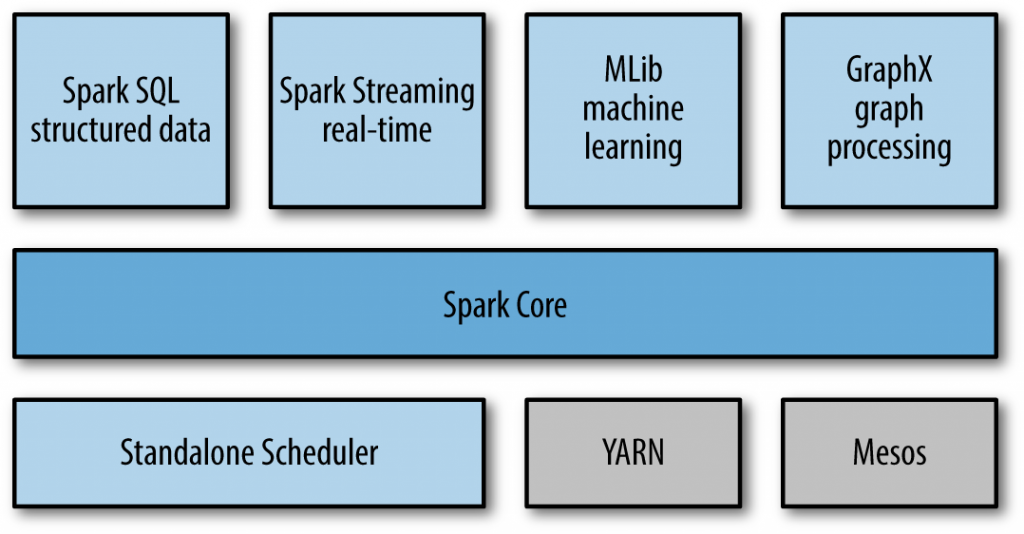
\includegraphics[width=1\textwidth]{img/sparkcore.png}
    \caption{Spark core e librerie}
    \label{fig:spark_core}
\end{figure}
\newpage



